% Created by tikzDevice version 0.12.6 on 2024-12-03 17:33:39
% !TEX encoding = UTF-8 Unicode
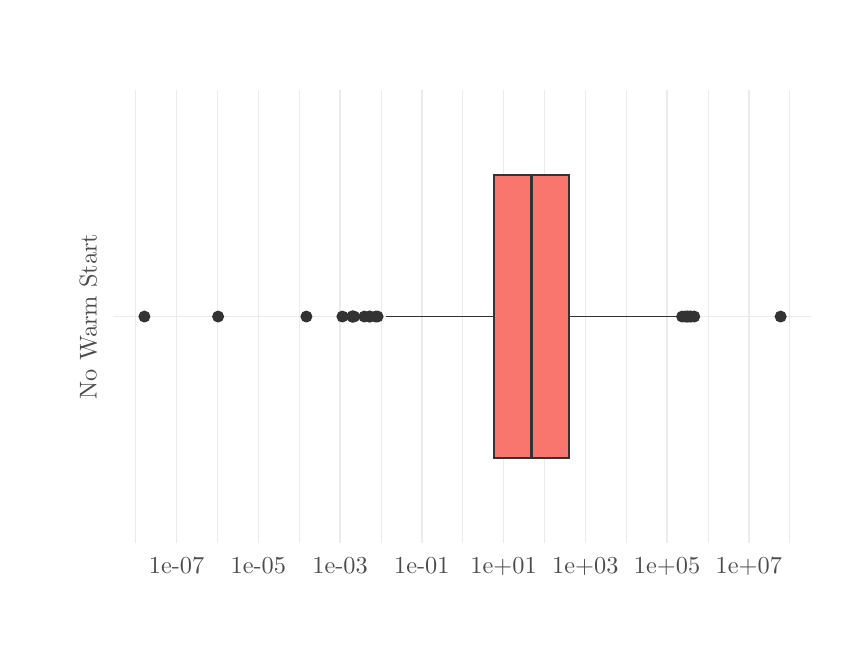
\begin{tikzpicture}[x=1pt,y=1pt]
\definecolor{fillColor}{RGB}{255,255,255}
\path[use as bounding box,fill=fillColor,fill opacity=0.00] (0,0) rectangle (289.08,216.81);
\begin{scope}
\path[clip] ( 30.69, 30.69) rectangle (283.58,194.15);
\definecolor{drawColor}{gray}{0.92}

\path[draw=drawColor,line width= 0.3pt,line join=round] ( 39.04, 30.69) --
	( 39.04,194.15);

\path[draw=drawColor,line width= 0.3pt,line join=round] ( 68.58, 30.69) --
	( 68.58,194.15);

\path[draw=drawColor,line width= 0.3pt,line join=round] ( 98.12, 30.69) --
	( 98.12,194.15);

\path[draw=drawColor,line width= 0.3pt,line join=round] (127.66, 30.69) --
	(127.66,194.15);

\path[draw=drawColor,line width= 0.3pt,line join=round] (157.20, 30.69) --
	(157.20,194.15);

\path[draw=drawColor,line width= 0.3pt,line join=round] (186.74, 30.69) --
	(186.74,194.15);

\path[draw=drawColor,line width= 0.3pt,line join=round] (216.28, 30.69) --
	(216.28,194.15);

\path[draw=drawColor,line width= 0.3pt,line join=round] (245.81, 30.69) --
	(245.81,194.15);

\path[draw=drawColor,line width= 0.3pt,line join=round] (275.35, 30.69) --
	(275.35,194.15);

\path[draw=drawColor,line width= 0.6pt,line join=round] ( 30.69,112.42) --
	(283.58,112.42);

\path[draw=drawColor,line width= 0.6pt,line join=round] ( 53.81, 30.69) --
	( 53.81,194.15);

\path[draw=drawColor,line width= 0.6pt,line join=round] ( 83.35, 30.69) --
	( 83.35,194.15);

\path[draw=drawColor,line width= 0.6pt,line join=round] (112.89, 30.69) --
	(112.89,194.15);

\path[draw=drawColor,line width= 0.6pt,line join=round] (142.43, 30.69) --
	(142.43,194.15);

\path[draw=drawColor,line width= 0.6pt,line join=round] (171.97, 30.69) --
	(171.97,194.15);

\path[draw=drawColor,line width= 0.6pt,line join=round] (201.51, 30.69) --
	(201.51,194.15);

\path[draw=drawColor,line width= 0.6pt,line join=round] (231.05, 30.69) --
	(231.05,194.15);

\path[draw=drawColor,line width= 0.6pt,line join=round] (260.58, 30.69) --
	(260.58,194.15);
\definecolor{drawColor}{gray}{0.20}
\definecolor{fillColor}{gray}{0.20}

\path[draw=drawColor,line width= 0.4pt,line join=round,line cap=round,fill=fillColor] (113.73,112.42) circle (  1.96);

\path[draw=drawColor,line width= 0.4pt,line join=round,line cap=round,fill=fillColor] ( 68.81,112.42) circle (  1.96);

\path[draw=drawColor,line width= 0.4pt,line join=round,line cap=round,fill=fillColor] (117.34,112.42) circle (  1.96);

\path[draw=drawColor,line width= 0.4pt,line join=round,line cap=round,fill=fillColor] (125.74,112.42) circle (  1.96);

\path[draw=drawColor,line width= 0.4pt,line join=round,line cap=round,fill=fillColor] (117.95,112.42) circle (  1.96);

\path[draw=drawColor,line width= 0.4pt,line join=round,line cap=round,fill=fillColor] (272.08,112.42) circle (  1.96);

\path[draw=drawColor,line width= 0.4pt,line join=round,line cap=round,fill=fillColor] (100.72,112.42) circle (  1.96);

\path[draw=drawColor,line width= 0.4pt,line join=round,line cap=round,fill=fillColor] (239.69,112.42) circle (  1.96);

\path[draw=drawColor,line width= 0.4pt,line join=round,line cap=round,fill=fillColor] (236.48,112.42) circle (  1.96);

\path[draw=drawColor,line width= 0.4pt,line join=round,line cap=round,fill=fillColor] (238.29,112.42) circle (  1.96);

\path[draw=drawColor,line width= 0.4pt,line join=round,line cap=round,fill=fillColor] (240.87,112.42) circle (  1.96);

\path[draw=drawColor,line width= 0.4pt,line join=round,line cap=round,fill=fillColor] (237.63,112.42) circle (  1.96);

\path[draw=drawColor,line width= 0.4pt,line join=round,line cap=round,fill=fillColor] (238.53,112.42) circle (  1.96);

\path[draw=drawColor,line width= 0.4pt,line join=round,line cap=round,fill=fillColor] ( 42.18,112.42) circle (  1.96);

\path[draw=drawColor,line width= 0.4pt,line join=round,line cap=round,fill=fillColor] (126.44,112.42) circle (  1.96);

\path[draw=drawColor,line width= 0.4pt,line join=round,line cap=round,fill=fillColor] (239.37,112.42) circle (  1.96);

\path[draw=drawColor,line width= 0.4pt,line join=round,line cap=round,fill=fillColor] (121.66,112.42) circle (  1.96);

\path[draw=drawColor,line width= 0.4pt,line join=round,line cap=round,fill=fillColor] (117.34,112.42) circle (  1.96);

\path[draw=drawColor,line width= 0.4pt,line join=round,line cap=round,fill=fillColor] (117.34,112.42) circle (  1.96);

\path[draw=drawColor,line width= 0.4pt,line join=round,line cap=round,fill=fillColor] (123.64,112.42) circle (  1.96);

\path[draw=drawColor,line width= 0.4pt,line join=round,line cap=round,fill=fillColor] (123.51,112.42) circle (  1.96);

\path[draw=drawColor,line width= 0.6pt,line join=round] (195.65,112.42) -- (236.28,112.42);

\path[draw=drawColor,line width= 0.6pt,line join=round] (168.52,112.42) -- (129.44,112.42);
\definecolor{fillColor}{RGB}{248,118,109}

\path[draw=drawColor,line width= 0.6pt,fill=fillColor] (195.65, 61.34) --
	(168.52, 61.34) --
	(168.52,163.50) --
	(195.65,163.50) --
	(195.65, 61.34) --
	cycle;

\path[draw=drawColor,line width= 1.1pt] (182.00, 61.34) -- (182.00,163.50);
\end{scope}
\begin{scope}
\path[clip] (  0.00,  0.00) rectangle (289.08,216.81);
\definecolor{drawColor}{gray}{0.30}

\node[text=drawColor,rotate= 90.00,anchor=base,inner sep=0pt, outer sep=0pt, scale=  0.88] at ( 24.88,112.42) {No Warm Start};
\end{scope}
\begin{scope}
\path[clip] (  0.00,  0.00) rectangle (289.08,216.81);
\definecolor{drawColor}{gray}{0.30}

\node[text=drawColor,anchor=base,inner sep=0pt, outer sep=0pt, scale=  0.88] at ( 53.81, 19.68) {1e-07};

\node[text=drawColor,anchor=base,inner sep=0pt, outer sep=0pt, scale=  0.88] at ( 83.35, 19.68) {1e-05};

\node[text=drawColor,anchor=base,inner sep=0pt, outer sep=0pt, scale=  0.88] at (112.89, 19.68) {1e-03};

\node[text=drawColor,anchor=base,inner sep=0pt, outer sep=0pt, scale=  0.88] at (142.43, 19.68) {1e-01};

\node[text=drawColor,anchor=base,inner sep=0pt, outer sep=0pt, scale=  0.88] at (171.97, 19.68) {1e+01};

\node[text=drawColor,anchor=base,inner sep=0pt, outer sep=0pt, scale=  0.88] at (201.51, 19.68) {1e+03};

\node[text=drawColor,anchor=base,inner sep=0pt, outer sep=0pt, scale=  0.88] at (231.05, 19.68) {1e+05};

\node[text=drawColor,anchor=base,inner sep=0pt, outer sep=0pt, scale=  0.88] at (260.58, 19.68) {1e+07};
\end{scope}
\end{tikzpicture}
